%!TEX root = ../dissertation.tex

%\begin{savequote}[75mm]
%Even two shoes in the box are correlated!
%\qauthor{Dr. Alexander Lukin}
%\end{savequote}

\chapter{Quantum gas microscope: \newline an overview}

\newpage

All experiments presented in this thesis are performed using an apparatus designed in a quantum gas microscope architecture for bosonic atoms.\footnote{Traditional microscope naming conventions typically refer to the method by which they probe the phenomena of interest (i.e. \emph{optical} microscopy, \emph{electron} microscopy). Although this microscope may seem dissimilar to this naming convention, an important point of this apparatus is that it is using the quantum properties of the degenerate atomic gas to probe physics that is harbored by Hamiltonians of interest. While I don't think this name was intentionally chosen to reflect this approach, I think it is an accurate description.} We study at a degenerate, quantum gas of $^{87}$Rb atoms in either one or two dimensions by confining the atoms to a single-plane in a three-dimensional optical lattice. This single-plane of ultracold atoms lies at the focus of an imaging system with a high numerical aperture (NA) of 0.8. The occupation of these lattice sites can be readout with single-site resolved resolution via an in-situ fluorescence imaging technique. A far more detailed description of this apparatus are provided in a number of other publications (ref people) and only the core components necessary to explain the successive work of this thesis will be explained here.  

\begin{figure}[ht!]
		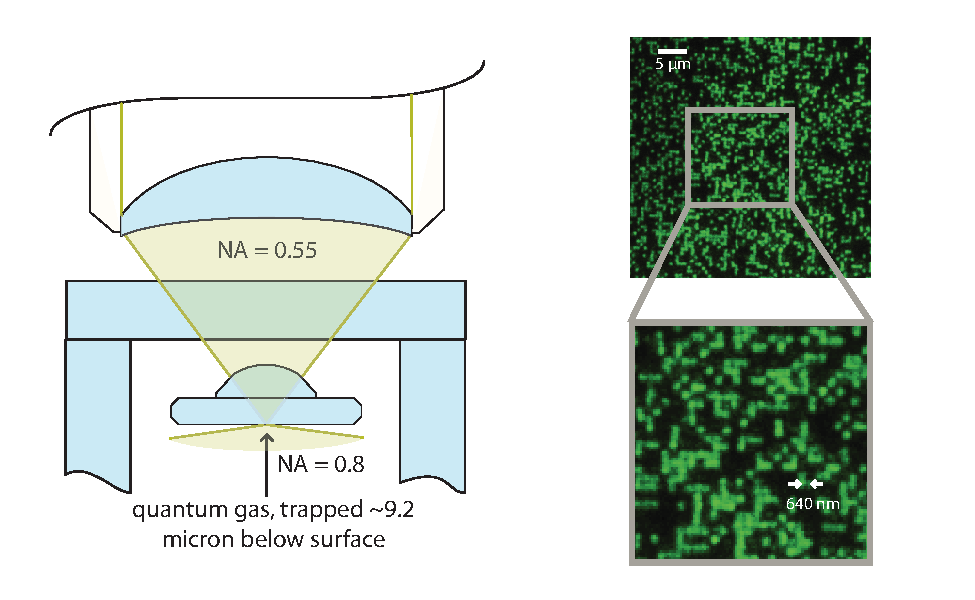
\includegraphics[width=\columnwidth]{figures/ch2/QGM/imaging_system_green.pdf} 
		\caption{\textbf{Schematic of Objective and Glass Cell. a,}  Heart of the quantum gas microscope }
		\label{fig:qgm}	
\end{figure}

While all ultracold atom machines are an amalgamation of many parts that collectively record the successes of atomic physics for the past several decades, the schematic in Fig.~\ref{fig:qgm} only represents the latest addition and the heart of the experimental apparatus. This schematic shows the high-NA imaging objective that sits outside an evacuated glass cell in which the degenerate quantum gas is formed. The custom objective that sits outside the glass cell has an NA $\approx 0.55$. The in-vacuum hemispherical lens is made of fused silica with a refractive index of $n=1.45$ and increases the combined NA to $\approx 0.8$.  We create a Bose-Einstein condensate (BEC) of $^{87}$Rb by conventional evaporation in a magnetic trap that resides at the focus of this imaging system which is $\approx 10\mu m$ below the bottom surface of the hemisphere. The $z$-confining lattices enter into the glass cell from the sides while the $x-y$ plane lattices are projected through the objective itself. The occupation of the lattice sites are imaged onto an EMCCD camera (ixon whatever) using fluorescence imaging from polarization gradient cooling via optical molasses beams. These two paths are the two generic options for optical access to the atoms and all other beams are combined onto these paths by either beam-splitters or dichroic filters.

\section{Optical lattice potentials}

The dominant potential landscape experienced by the atoms is defined by optical lattices in three dimensions. The atoms are loaded from the BEC in a magnetic trap into a single two-dimension plane by being confined by a single node of a vertical ($z$-direction) lattice. All studied physics relating to the Bose-Hubbard model derived in the previous chapter is restricted to within this two-dimension plane ($x,y$-direction). All lattices are formed by interfering two beams a long a given axis which produces a square lattice in all directions with a sinusoidal shape.


MAKE STATEMENT ABOUT PHOTODIODES SOMEWEHRE?

\subsection{$z$-Lattices}

The loading of the BEC into a single node of the $z$-confining lattices is conducted via a two-step process and requires two different $z$ lattices. Both of these lattices are generated from a single beam that is reflected off the uncoated, flat surface of the hemispherical, in-vacuum lens as shown in Fig.~\ref{fig:qgm}. 

The first step comes from a beam illuminating this surface from a very shallow angle and forms a large spacing lattice with a lattice constant of $\approx 9.2 \mathrm{\mu m}$ which corresponds to a recoil energy $E_r \approx 2 \pi \times 7$ Hz. This large spacing lattice is denoted as the ``big" lattice. The atoms are loaded into the 1$^{st}$ minimum of the lattice from this surface, which provides the reference for defining all $z$-positions in the apparatus. While this bottom surface is uncoated, the angle is sufficiently shallow ($\approx 88^\circ$ from normal) such that the Fresnel intensity reflection coefficient is reasonably large ($R_s\approx  0.85$). This reflection coefficient produces a lattice with a  contrast of $\approx 0.997$. This means that for a measured lattice depth of $V_o^{big}$, the corresponding DC offset will be $\approx 0.002 \times V_o^{big}$.

The second step involves a hand-off with a second beam that illuminates the surface from the opposite direction at a less shallow angle ($\approx 75.6^\circ$) to produce a lattice with a smaller lattice constant of $\approx 1.5 \mathrm{\mu m}$ which corresponds to a recoil energy $E_r \approx 2 \pi \times 255$Hz. This smaller spacing lattice is denoted as the ``axial" lattice. The atoms lie in the 6$^{th}$ minimum of this lattice which overlaps with 1$^{st}$ minimum of the ``big" lattice. The uncoated surface has a more detrimental effect at this illumination angle where the Fresnel intensity reflection coefficient is much significantly smaller ($R_s \approx 0.39$). However, since the beam interferes with itself upon reflection, the interference contrast still remains relatively high at $\approx 0.90$. This means for a measured lattice depth of $V_o^{axial}$, the corresponding DC offset will be $\approx 0.056 \times V_o^{axial}$. The angle dependencies of both of these parameters, minimum offset and contrast, are plotted in Fig.~\ref{fig:axLatt}.

\begin{figure}[ht!]
		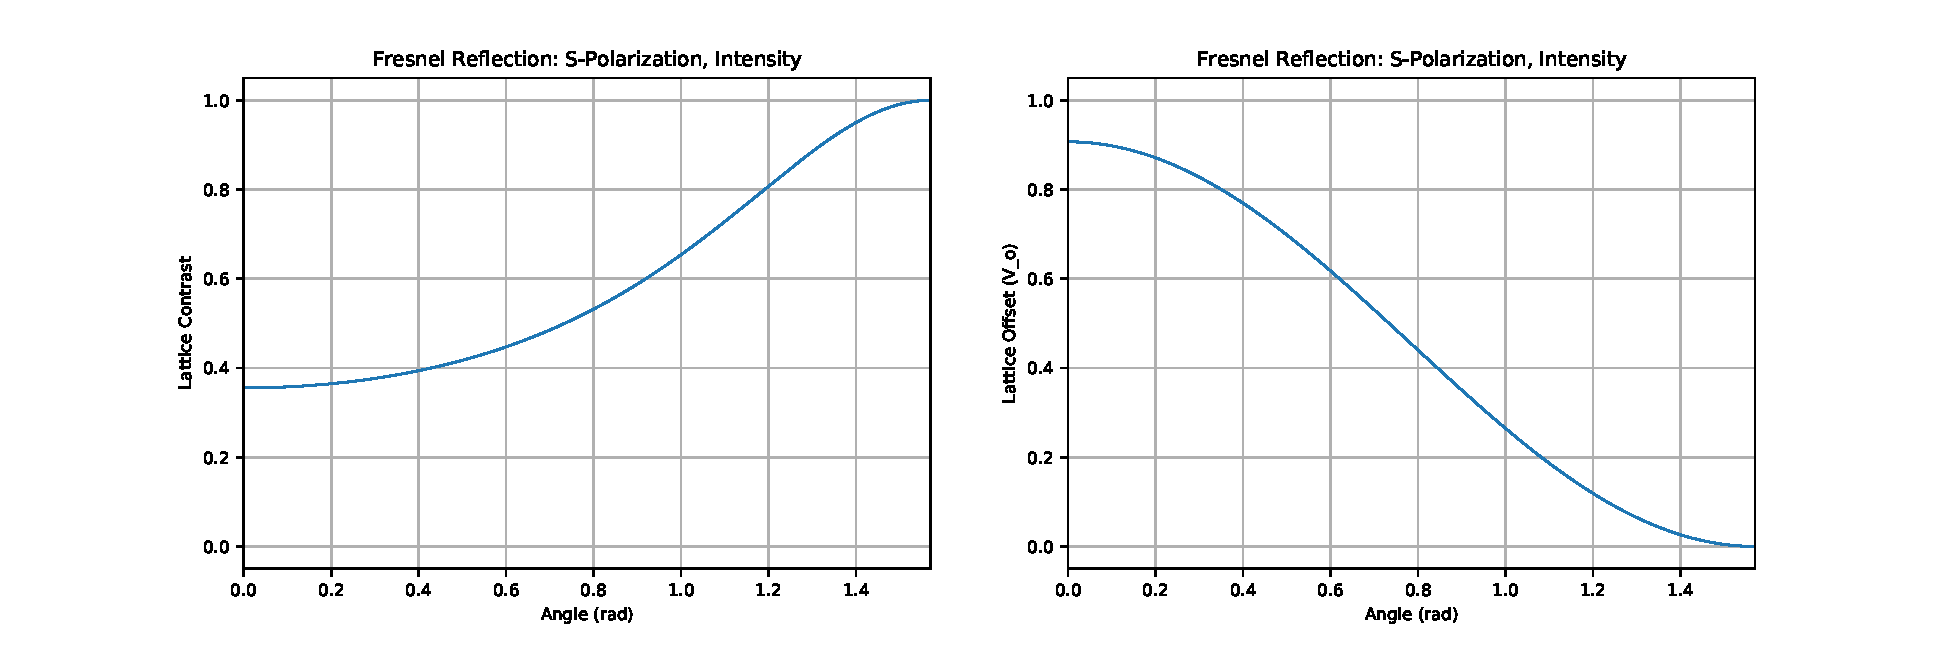
\includegraphics[width=\columnwidth]{figures/ch2/heating_rates/axLatRef.pdf} 
		\caption{\textbf{Lattice Parameters vs. Angle Rate a,} Lattice Contrast \textbf{b,} offset in units of lattice depth }
		\label{fig:axLatt}	
\end{figure}

Both of these $z$-confining lattices are generated from an amplified Superluminescent Light Emitting Diode (SLED) source centered at $\lambda \approx 755 nm$. The bandwidth of this light is relatively wide $\approx 3 \mathrm{nm}$ such that the light is approximately temporally \emph{in}coherent. The corresponding coherence length is $\approx 100 \mathrm{\mu m}$which is much longer than the $z$-lattice spacing and allows for relatively high-contrast interference quoted above. This short coherence length, while allowing the creation of a high contrast lattice at the length scales of interest, it prevents interference of any of the conservative potential beams with one another or with reflections from surfaces more than $100 \mathrm{\mu m}$ away.

\subsection{$x,y$-Lattices}

In the $x-y$ plane, the lattices are imaged onto the atoms from a holographic mask through the objective (Fig.~\ref{fig:qgm}). The spacing of this lattice is $\approx 680$ nm which corresponds to a recoil energy $E_r \approx 2 \pi \times 1240 Hz$. The holographic mask is a phase hologram that imprints a square wave of alternating $0$ and $\pi$ phase onto the profile of the illuminating beam. This phase imprint nearly eliminates the 0$^{th}$ order light emanating from the hologram and only the $\pm1$ orders are imaged on to the atoms. This produces a sinusoidal lattice with relatively high contrast due to the satisfaction of the imaging condition in the microscope. However, it additionally means that any unwanted artifacts (e.g. dust on the hologram) is additionally imaged onto the atom potential and creates local disorder. To alleviate some of this disorder, the beams are spatially filtered in the Fourier plane of the imaging system (cite 72 from philipp).

The same SLED source used to produce the $z$-confining lattices is also used to produce these lattices in the $x-y$ plane. Since the lattices are imaged onto the atoms, a more temporally incoherent source could, in principle, be used.

\subsection{Disorder (unintentional) and heating rates} \label{sec:ch2_heating}

The use of temporally incoherent light alleviates the contribution of stray reflections to unwanted interference, and hence unwanted disorder, in the system. However, since the lattices themselves are imaged from a holographic mask onto the atoms, the fidelity of the lattice potentials is very sensitive to local scatters in the image plane of the imaging system. There are two approaches to alleviate this problem: spatial filtering of the lattice beams in the Fourier plane of the system (currently implemented), or the illumination of the mask with spatially incoherent light that would average out any local scatterer.

Within the context of a faithful realization of the Bose-Hubbard model, the dominant effect from this disorder corresponds to a modulation in the on-site potential height $h_i$ in the tight-binding limit. However, the choice of blue- or red-detuned lattices affect the relationship of $h_i$ to the actual intensity of the scattered beam. In the case of red-detuned lattices, the atoms reside at the intensity maxima which means that, in the tight-binding limit, the on-site potential contains both the lattice depth $-V_o$ and the zero-point energy $\propto V^{1/2} \propto \hbar \omega_{ho}/2$. In a blue-detuned lattice, the atoms reside at the intensity minima and hence are sensitive to only the zero-point energy shift $\propto V^{1/2}$. This dependence is plotted in Fig.~\ref{fig:epsV} as a function of scattered intensity $\epsilon$ difference between two beams interfering to produce the optical lattice. The light used to produce the lattices potentials in the experiment has a center frequency of $\lambda=755$ nm which is far blue-detuned from atomic resonances of $\lambda_{D1} = 795$ nm and $\lambda_{D2}=780$ nm. 

The other relevant consideration for the faithful realization of the Bose-Hubbard model in optical lattices depends on residual spontaneous scattering of light from the lattices by the atoms. This light will necessarily impart some kinetic energy onto the atom and begin to populate higher bands in the lattice. This may appear, at first glance, to not be a significant issue in the case of a blue-detuned lattice since the atoms sit at the intensity minima. While the scattering rate is indeed significantly different for the blue- and red-detuned cases, the ``heating" rate (rate at which atomic population is moved to higher bands) is not necessarily different (cite daley paper). This result of equivalent ``heating" for both blue- and red-detuned lattices corresponds only to the increase in average energy for an atom. However, it doesn't take into account the increase in entropy related to the dephasing of a many-body state evolving under the Bose-Hubbard model. This will become the metric of interest and therefore the scattering rate the more appropriate quantity for comparing between lattice detunings (Fig.~\ref{fig:heating}).

We compare several methods for calculating the spontaneous scattering rate in the lattice. The first estimate that will be considered follows an assumption of deep lattices and being deep within the Lamb Dicke regime (cite Daley). Once you include the Lamb Dicke parameter,  $\eta^2=(4V_o/E_r)^{-1/2}$, the estimated heating rate for deep lattices is just:

\begin{equation}
\gamma=E_r \frac{\Gamma}{2 \Delta} \left ( \frac{V_o}{E_r}  \right )^{1/2}
\label{eqn:lambDickeEst}
\end{equation}

where $\Gamma$ is the linewidth of the D2 transition (nearest resonance for the blue lattice), $\Delta$ is the detuning of the lattice light from the D2 transition, and $E_r$ is the lattice recoil energy. In the case of the $x-y$ lattices, which should have no appreciable offset, this will become a good estimate of the spontaneous scattering rate as shown in Fig.~\ref{fig:heating}. However, it is a poor description of the spontaneous scattering rate with an offset and so we take a more general approach that allows additional potential offsets (\ref{eqn:sponSc}).

\begin{equation}
\gamma=E_r \frac{\Gamma}{\Delta} \int~dx~ \left ( V_{latt}(x) + V_{offset} \right ) |\psi(x)|^2
\label{eqn:sponSc}
\end{equation}

where the considered $\psi(x)$ is either the Wannier wavefunctions, $w_n(x)$, or the Harmonic Oscillator wavefunctions. These more accurate estimates from (\ref{eqn:sponSc}) are plotted in Fig.~\ref{fig:heating}. The relevant lattice depths are: $\approx 2-45E_r^{x,y}$ for the $x-y$ lattices, $\approx 40-250 E_r^{axial}$ for the axial lattice, and $\approx 3,000-20,000 E_r^{big}$ for the big lattice.

\begin{figure}[ht!]
		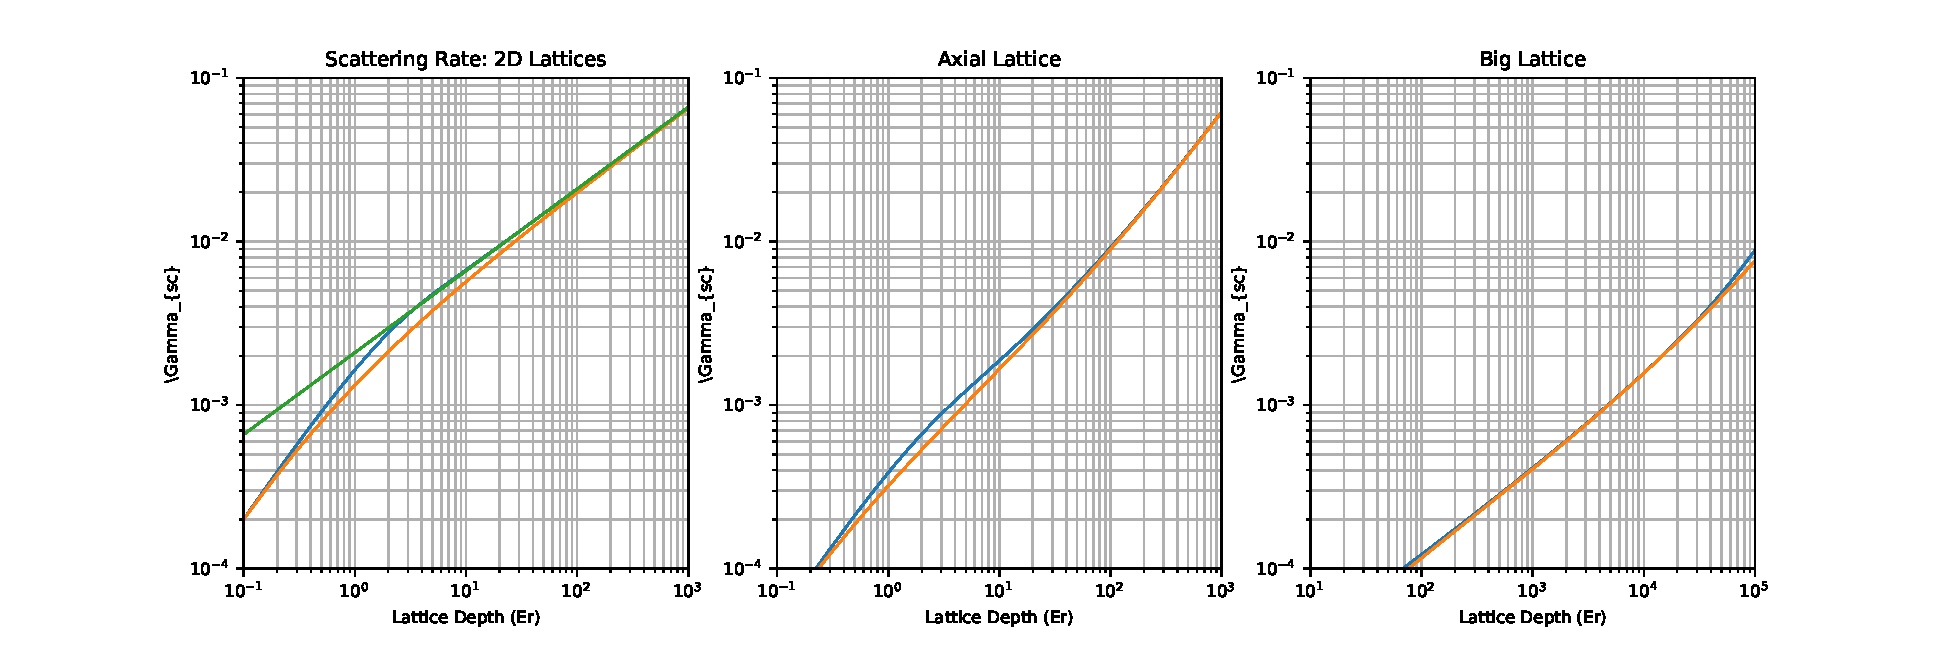
\includegraphics[width=\columnwidth]{figures/ch2/heating_rates/ScatteringRates.pdf} 
		\caption{\textbf{Spontaneous Scattering Rate a,}  2D \textbf{b,} Axial, \textbf{c,} Big }
		\label{fig:heating}	
\end{figure}

Could make this statement that for the same scattering rate at the same lattice depth, you need to detune a red lattice such that $\Delta_R = \Delta_B (1+\eta^2)/\eta^2 = \Delta_B \left ( 1 + \left ( \frac{E_r}{4 V_o} \right )^{1/2}  \right ) \left ( \frac{E_r}{4 V_o} \right )^{1/2} $

Lifetime from background collisions is $\approx 33(3)$s. 


\section{Arbitrary potential generation}

The ability to realize interacting, many-body systems at ultracold temperatures has been the work horse of atomic gasses and allows the observation exotic physics such as the superfluid to Mott-insulator transition (cite markus and people). The addition of a microscope to these systems enables single-site resolution and access to the lattice sites in the system. Not only can this be used for imaging to determine which lattice sites are occupied by atoms, but by symmetry enables the microscope to be used in reverse to project local optical potentials on the order of a lattice site.

Using this capability for single-site optical potential projection has enabled a series of pioneering experiments that enable Hamiltonian engineering on top of the bare Bose-Hubbard model. This is implemented in our apparatus via a Digital Micromirror Device (DMD) that is located in the Fourier plane of our imaging system. Even though the DMD only provides a binary mask for projecting patterns onto the atoms, the fact that it is in the Fourier plane enables finer resolution for single-site features that are spread out across a significant portion of the DMD. Only a brief description of this setup will be mentioned here such that it provides context for how it is used in the successive experiments detailed in this thesis. A more detailed description of this setup can be found in the theses are article (ref other theses for technical details + philip zupancic paper).

The DMD is illuminated with a laser that is blue-detuned from the D1 and D2 transitions with a center wavelength $\lambda_{DMD} = 765$ nm. By placing the DMD in the Fourier plane of the imaging system, all desired potentials must be programmed as the Fourier transform of the desired potential at the atom plane. Additionally, the potential generation on the DMD incorporates an additional grating in the projection that allows for both amplitude and phase control of the light. Since it is really the \emph{field} of the light that is tunable with the DMD, the patterns produced can be pre-compensated for aberrations in the imaging system such that the desired potentials is produced to a high fidelity. Aberrations in this system can be reduced to $\approx \lambda/10$ at the atom plane.

\subsection{Disorder (intentional)}

The DMD is used for two primary functions for the experiments in this thesis: 1) wall-like potentials that act to isolate sections of the optical lattices and 2) the generation of local, tunable ``disorder" for the realization of localized states in the Bose-Hubbard model. For all experiments in this thesis the applied potential used to localize the wavefunctions is sampled from a quasi-periodic distribution of on-site potentials.  

\section{Imaging and readout}

At the end of every experimental sequence, the atoms are imaged via fluorescence imaging by optical molasses beams. The recoil of this near-resonant light necessarily and significantly excites the atoms to higher-bands in the optical lattice. Even though the optical molasses light provides polarization gradient cooling, the average energy would not remain trapped in the far from resonant lattices used for studying Bose-Hubbard model physics. To keep the atoms trapped to a single lattice site during imaging we use near-resonant lattices that are blue-detuned by $\approx 55$ GHz from the $\lambda_{D1} = 795$ nm transition. The depth of this ``imaging" or ``pinning" lattice is $\approx 5000 E_r$. This light is generated by a verdi bla bla bla. 

During the flourescence imaging process, an additional complication occurs for multiply occupied sites. The absorption of a photon by the atom leads to the formation of an electron dipole moment from the excited state. This, in turn, induces a dipole into a nearby atom on the same lattice site such that they form a molecular potential and causes the atoms to gain kinetic energy via their mutual attraction. However, the excited state will then decay on the order of linewidth. This process will quickly leave both atoms with enough energy to escape even the deep imaging lattice and is known as photo-assisted collisions (cite people). Importantly, this results in pair-wise loss from a lattice site during imaging such that only the parity of the on-site occupation number is image and is known as ``parity projection."

This parity projection imaging can be circumvented for one-dimensional slices of the lattice by using the DMD. The DMD is used to create two wall-like potentials that isolated a single row or column of the lattice. The corresponding lattice is then reduced in depth such that all other atoms outside of this isolated tube escape the system. Then the atoms within isolated tube are expanded along the orthogonal direction for a brief time such that they are very spread out over the orthogonal direction during the imaging sequence. This makes it very unlikely, in a probabilistic sense, for the atoms to occupy the same site and be ejected from the lattice due to the photo-assisted collisions. This expansion allows for on-site occupation number resolution. For a one-dimensional, many-body wavefunctions this amounts to a projective measurement on the particle number basis or Fock basis. 

This resolution of the on-site number distribution enables several important key features for probing quantum many-body systems. It enables readout of the entire diagonal of full system's density matrix which allows for probing correlations within this basis. It also enables higher-fidelity state readout in two ways: during the imaging process there is a finite probability an atom hops to a neighboring site which can result in photo-assisted collisions and it also enables post-selection on total atom number. The former of these two considerations is shown by comparing the in-situ (parity projected) image versus the full counting image of a Mott-insulator (Fig.~\ref{fig:MIFC}). The latter is an essential tool for reducing the heating that contributes to measurements in the experiments described later on in this thesis.

\section{Calibration of energy scales}

The ability to accurately determine all experimental parameters in the system is an invaluable benefit to the precision of the results generated by this experiment. I have briefly described many of the import calibration steps that were used ubiquitously throughout this thesis to accurately determine Bose-Hubbard parameters for conducting experiments and will not be described otherwise. Additionally, many of these methods are built upon previous results using the apparatus and in some cases are throughly detailed in those publications, which will be cited in the appropriate locations.


\subsection{Lattice depth: Kapitza-Dirac Scattering}

A particularly efficient method to calibrate the lattice depth experienced by the atoms is via Kapitza-Dirac scattering (cite gretchen campbell etc). This method requires that the atoms have Bose-condensed so that their many-body wavefunction has a well defined phase across the entire cloud. The lattice is then turned on very diabatically\footnote{This means the new Hamiltonian is turned on significantly faster than all the inverse energy scales in the system such the wavefunction itself has not evolved during the turn on time.} and illuminates the atoms for a variable, but brief time period. This brief illumination of the atoms is such that the atoms only experience a potential that evolve the local phase of their wavefunction but the atoms have not had time to move yet. The imprinted phase on the atoms has a spatial structure that is proportional to the lattice potential and can be probed easily via common time of flight measurements which map the spatial Fourier components, or wavevectors of the wavefunction, to momentum. 

This mapping of the imprinted spatial phase on the BEC to momentum has a convenient and clean analytical form that results from the spatial phase always being commensurate with periodicity of the lattice. This results in the atomic momentum only being non-zero at integer multiples of the lattice wavevector. The population in these integer multiples then follows the analytic form given by:

\begin{equation}
\label{eqn:KDanalytic}
P_{|\nu|}(t)= \left | \mathcal{J}_\nu \left ( \pi E_r \frac{V_o}{E_r} t \right ) \right |^2
\end{equation}

where $\mathcal{J}_\nu$ is the Bessel function of the1$^{st}$ kind, $\nu$ denotes the integer of the lattice vector and the order of the Bessel function, $V_o$ is the lattice depth in Hz, $E_r$ denotes the recoil energy of the lattice, and $t$ is the time the atoms have evolved in the presence of the lattice. The derivation of this form is shown in Appendix \ref{appendix:Ch2Cal}. The evolution of the population into these modes is shown as a function of time in Fig.~\ref{fig:KDScatt}. As can be seen in this figure, the dynamics stop following the predicted evolution due to the presence of the additional trap confinement and that the wavefunction will also begin to redistribute atomic population in the presence of this lattice on the order of the local, lattice site trap frequency $\omega_{Latt}$.

\begin{figure}[ht!]
		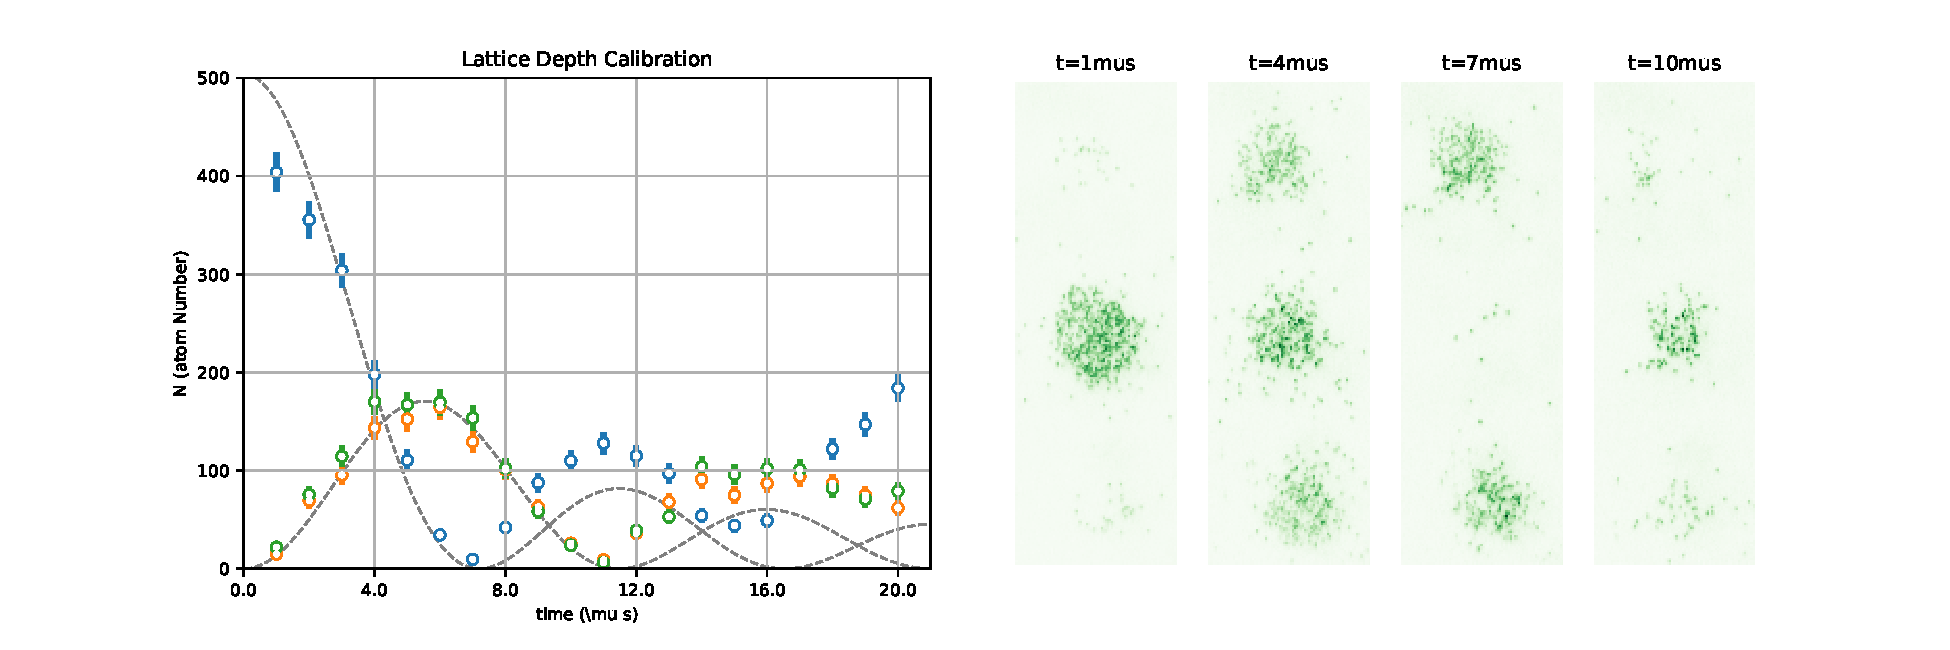
\includegraphics[width=\columnwidth]{figures/ch2/kapitza_dirac_latt_depth/KDCal.pdf} 
		\caption{\textbf{Kapitza-Dirac Scattering a,}   }
		\label{fig:KDScatt}	
\end{figure}

\subsection{Tunneling $J$ : single-atom quantum walks}

The tunneling matrix element( tunneling strength), $J$, can be calibrated from the quantum walk of single atoms in 1-D lattices. This protocol involves first isolating a single-atom at a particular site per 1-D lattice. These dynamics have been explore extensively in a number papers (cite Philipp, Yoav, and photon people) and of significant interest in their own right. While the tunneling strength and the lattice depth have a well defined theoretical relationship that could make this calibration seem redundant, practically speaking this method provides a far more accurate estimate of the local tunneling strength.\footnote{This is partially due to some of the systematic biases in the lattice depth calibration that uses Kapitza-Dirac scattering that limit the precision of the measurement. However, the other issue is that the optical lattices used in this apparatus have local variation in disorder that can locally modify the tunneling strength $J$. Since the vast majority of experiments in this system work with appreciably large-lattice depths and small systems, this is a significant consideration for calibrating experimental parameters.}  The analytic form is quite similar to the Kapitza-Dirac scattering form (this is not by accident, please refer to the derivations in Appendix \ref{appendix:Ch2Cal}):

\begin{equation}
\label{eqn:QWanalytic}
P_{|\nu|}(t)= \left | \mathcal{J}_\nu \left ( {2 \times  2 \pi J t} \right ) \right |^2
\end{equation}

where $\mathcal{J}_\nu$ is the Bessel function of the1$^{st}$ kind, $\nu$ denotes the integer of the lattice vector and the order of the Bessel function, and $J$ is the tunneling strength. There is an additional formulation that includes the possibility for local potential gradients that can provide a better fit and is the corresponding from for what are known as Bloch oscillations:

\begin{equation}
\label{eqn:BlochOsc}
P_{|\nu|}(t)= \left | \mathcal{J}_\nu \left (  \frac{2 J}{\pi E} \sin \left( {\pi E t / h}\right ) \right ) \right |^2
\end{equation}

where $E$ is the local potential gradient. For a given evolution time $t$, a corresponding lattice size can be fit where $ |\nu| \leq L/(2 \pi J) $. \footnote{This bound is determined by the Lieb-Robinson bound, which for a single-atom in a lattice is determined by the steepest slope (maximum group velocity) of its corresponding band.} Theses fits and averaged site-occupation date are shown in Fig.~\ref{fig:QWCal}. Note that at very low-lattice depths, the tight-binding, nearest-neighbor coupled Bose-Hubbard model becomes a less accurate description of the physics in the lattice and hence higher-order tunneling terms become significant. The deviation, both theoretical an measured, is shown in the figure.

\begin{figure}[h!]
		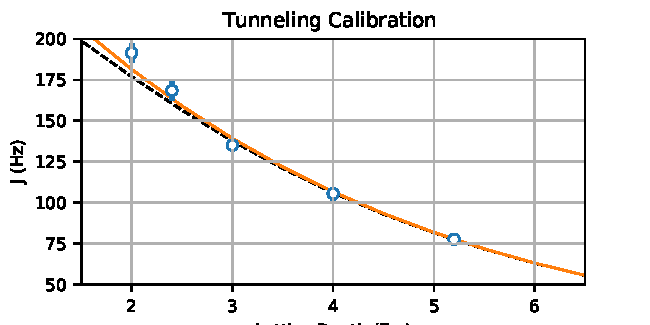
\includegraphics[width=3.5 in ]{figures/ch2/QW_cal/QWCal.pdf} 
		\caption{\textbf{Quantum Walk a,}   }
		\label{fig:QWCal}	
\end{figure}



\subsection{Interaction $U$ and linear tilt $E$: photon-assisted tunneling} \label{sec:EUcal}

Determining the interaction strength $U$ and local potential variation from disorder can be determined from a single protocol that utilizes photon-assisted tunneling (cite alex ma and others). This method first starts from deep in a Mott-insulating regime where there is exactly an integer number of atoms per lattice site. Then a potential gradient is applied to the system such that increases the on-site potential energy by $E$ Hz per site that is larger than the interaction energy $U$. Then the lattice depth is lowered to  intermediate lattice depth $\approx 15 E_r$ where the tunneling $J$ is still much smaller than $U$ or $E$. The lattice depth is then modulated at small amplitude at various frequencies to restore tunneling between the sites that are currently far away from resonance. When the frequency matches the energy difference between two sites, it restores tunneling and appears as fluctuations away from the Mott-insulating state.

There is a useful asymmetry in this protocol due to the on-site interactions. In the regime where $E>U$, the energy difference for an atom to hop to neighboring sites will cost either $E+U$ or $E-U$ energy depending on the direction of increasing gradient potential. This means that by measuring out both resonance conditions both $E$ and $U$ can be calibrated locally.  This is demonstrated in Fig.~\ref{fig:EUCal} where the two resonances are measured, and the variance of the tilt $E$ and the interaction $U$ across the measured region reveal residual on-site disorder and on-site curvature. 

\begin{figure}[h!]
		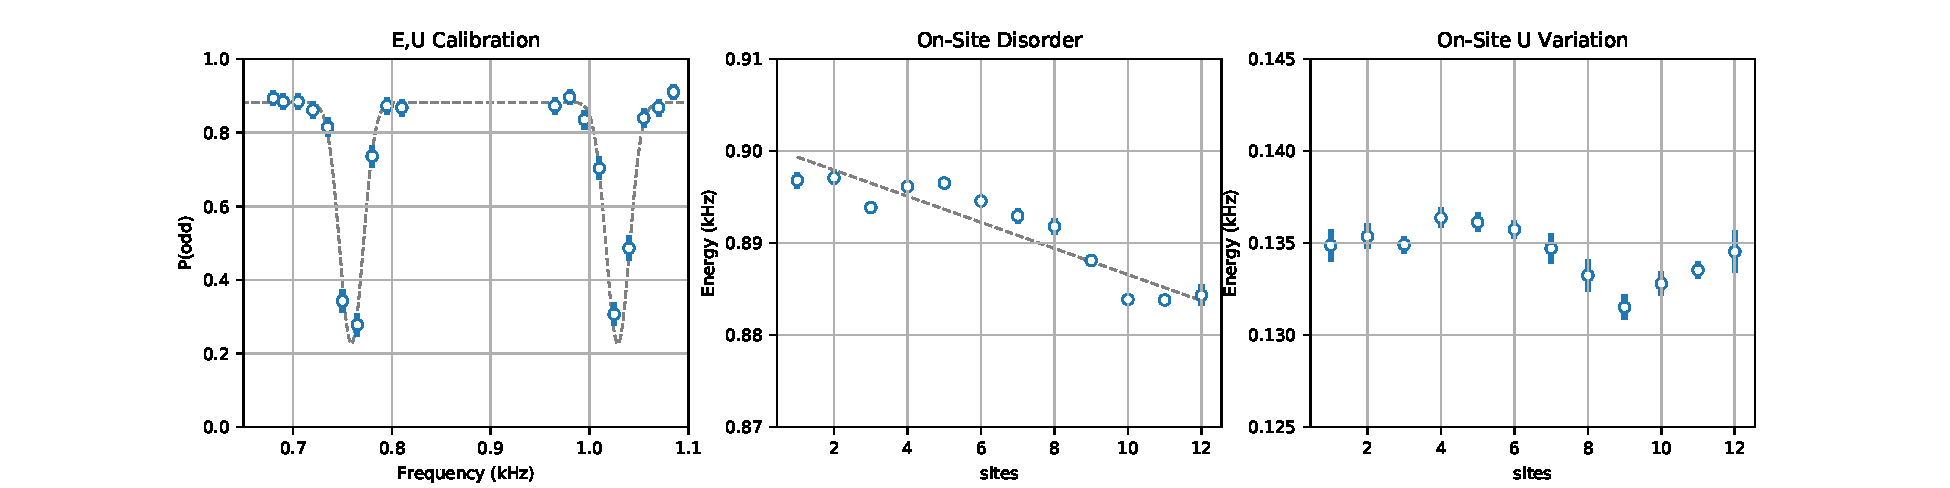
\includegraphics[width=\columnwidth]{figures/ch2/E_U_cal/EUCal.pdf} 
		\caption{\textbf{Calibrate Interaction and Tilt a,}  2D \textbf{b,} Variation of tilt, curvature of offset, \textbf{c,} Variation of interaction, variation of on-site curvature }
		\label{fig:EUCal}	
\end{figure}

\begin{figure}[h!]
		\includegraphics[width=\columnwidth]{figures/ch2/E_U_cal/UCal.pdf} 
		\caption{\textbf{Calibrate Interaction and Tilt  2a,}  2D \textbf{b,} COMBINE FIGURES }
		\label{fig:EUCal}	
\end{figure}

While the tilt $E$ here is described as purely a part of a process that is necessary to suppress tunneling such that  $U$ and on-site differences can be measured, the tilt itself is also sometimes the quantity of interest. In some experimental schemes that implement synthetic magnetic fields in ultracold atom experiments, a potential gradient is used to suppress the bare, resonant tunneling in the lattice $J$ along one direction which is then restored with a spatially varying phase. This has been explored in several cold atom experiments (cite bloch and ketterle people) and was implemented in this system to probe the Harper-Hofstadter model (cite erics paper) and is described in significant detail here (eric's thesis).

\subsection{On-site Disorder pattern $h_i$ : adiabatic transfer}

The generation of single-site resolved potentials $h_i$ are created via the DMD installed in the apparatus and are used extensively for state initialization and site-occupation read out during imaging. However, in both of these cases, the absolute depth of the potentials used is not particularly important since both procedures are relatively insensitive to them. However, some of the experiments in this thesis rely on a particular relationship of the on-site potential offsets $h_i$, to both the tunneling strength $J$ and interaction strength $U$. By calibrating these potential offsets using the atoms we can both compare how precisely the DMD can produce a desired optical potential and the absolute height of these potential in Hz.

We used a similar protocol to the $U$ calibration method mentioned above in \S \ref{sec:EUcal} and is similar a hybrid of the protocols used in previous studies (cite photon assited tunneling and ising paper). The method starts with a unity-filled Mott-insulating state. A tilt of strength $E$ Hz/site is then applied to the system to bring all sites far from resonance with their neighbors. The lattice depth is then reduced to an intermediate depth with appreciable but small tunneling. The additional potential pattern is then turned on approximately adiabatically with respect to only the nearest neighbor tunneling strength $J$. Since the potential that is applied has varying on-site potentials $h_i$, the resonsance condition is again re-established when the energy difference between neighboring sites, $\Delta_i = h_i - h_{i-1}$, compensates for the energy offset $E-U$. The signal is to then find when the average on-site occupation changes from $n=1$ atom to $n=0,2$. This is actually measured in-situ as a change in parity. The example for this method shown in Fig.~\ref{fig:WCal} is performed for an on-site potential sampled from a quasi-periodic distribution: $h_i = W \cos{\left ( \beta 2 \pi i + \phi_o \right ) }$, where $\beta$ is the golden ratio $\approx 1.618$, $i$ is the site-index, and $\phi_o$ is an arbitrary phase factor.

\begin{figure}[h!]
		\includegraphics[width=\columnwidth]{figures/ch2/disorder_cal/WCal.pdf} 
		\caption{\textbf{Calibrate Disorder .. on-sit epotential 2a,}  2D \textbf{b,} COMBINE FIGURES }
		\label{fig:WCal}	
\end{figure}

This protocol is also described in the supplementary of this paper (cite MBL).

\subsection{Heating rates : spontaneous scattering}

As discussed earlier in \S \ref{sec:ch2_heating}, the spontaneous scattering rate provides a limit on the lifetime of many-body coherent processes. To estimate this limit, we determine the contribution of the spontaneous scattering rates present from all the confining optical potentials in the system. The approximate background lifetime related to background collisions with hot atoms (this is related to the vacuum quality in the glass cell) is a lifetime of $\tau_{Bkg} = 33(3)$s or scattering rate $\gamma_{Bkg} = 0.03(3)$ Hz. By measuring the atom loss late from relatively weak traps as a function of optical potential depth, we can measure the contribution of the additional optical potential to heating and the offset that comes from background gas collisions. In general, this loss will follow an exponential form $\sim n(t) = N_o e^{-\gamma_{Bkg} t - \gamma_{Optical}(v) t}$. By holding the atoms in just an optical harmonic potential and the axial confinement lattice, we were able to find good agreement with the predicted spontaneous scattering rate and the approximate background collision rate estimated by previous works (Fig.~\ref{fig:heatingCal}).(cite theses). This measurements put an approximate single-atom lifetime for all experiments in this thesis to be $\tau_{comb.-ax} \approx 14$s in the axial-lattice configuration and $\tau_{comb.-big} \approx 19$s in the big-lattice configuration.

\begin{figure}[h!]
		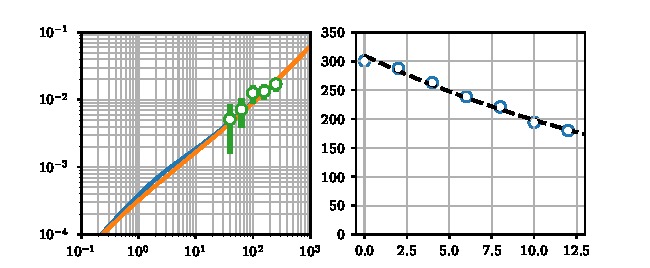
\includegraphics[width=3.5in]{figures/ch2/heating_rates/ScatteringRatesCal.pdf} 
		\caption{\textbf{Axial Lattice Heating Rate a,}   ADD INSITU PICTURE TO MAKE IT CLEARER + EXP DECAY}
		\label{fig:heatingCal}	
\end{figure}

\subsection{MI to SF heating? THINK ABOUT THIS LATER}

